\let\negmedspace\undefined
\let\negthickspace\undefined
\documentclass[journal]{IEEEtran}
\usepackage[a5paper, margin=10mm, onecolumn]{geometry}
%\usepackage{lmodern} 
\usepackage{tfrupee} 

\setlength{\headheight}{1cm} 
\setlength{\headsep}{0mm}     

\usepackage{gvv-book}
\usepackage{gvv}
\usepackage{cite}
\usepackage{amsmath,amssymb,amsfonts,amsthm}
\usepackage{algorithmic}
\usepackage{graphicx}
\usepackage{textcomp}
\usepackage{xcolor}
\usepackage{txfonts}
\usepackage{listings}
\usepackage{enumitem}
\usepackage{mathtools}
\usepackage{gensymb}
\usepackage{comment}
\usepackage[breaklinks=true]{hyperref}
\usepackage{tkz-euclide} 
\usepackage{listings}                                        
\def\inputGnumericTable{}                                 
\usepackage[latin1]{inputenc}                                
\usepackage{color}                                            
\usepackage{array}                                            
\usepackage{longtable}                                       
\usepackage{calc}                                             
\usepackage{multirow}                                         
\usepackage{hhline}                                           
\usepackage{ifthen}                                           
\usepackage{lscape}

\begin{document}

\bibliographystyle{IEEEtran}
\vspace{3cm}

\title{4.12.8}
\author{AI25BTECH11003 - Bhavesh Gaikwad}
{\let\newpage\relax\maketitle}

\renewcommand{\thefigure}{\theenumi}
\renewcommand{\thetable}{\theenumi}
\setlength{\intextsep}{10pt} 


\numberwithin{equation}{enumi}
\numberwithin{figure}{enumi}
\renewcommand{\thetable}{\theenumi}


\textbf{Question}: Distance of the point $(\alpha, \beta, \gamma)$ from y-axis is\\
a) $\beta$\\
b) $|\beta|$\\
c) $|\beta + \gamma|$\\
d)$\sqrt{\alpha^2 + \gamma^2}$ \\

\textbf{Solution:}\\
Let $\vec{A} = \myvec{\alpha \\ \beta \\ \gamma}$\\
Let $\vec{B}$ be the point on y-axis which is nearest to $\vec{A}$.\\


\begin{equation}
\text{Equation of y-axis: } \vec{r} = \lambda \vec{e_2}, \, where \, e_2=\myvec{0 \\ 1 \\ 0}
\end{equation}


Since point $\vec{B}$ satisfies the equation,
\begin{equation}
    \vec{B} = \lambda \vec{e_2}
\end{equation}\\

$\vec{(B-A)}$ is perpendicular to the y-axis as its the shortest distance between a line and a point $\vec{A}$ or $\vec{B-A}$ is perpendicular to $\vec{B}$ as it lies on the y-axis itself.

\begin{equation}
    \therefore \, \vec{(B-A)}^\top\vec{B} = 0
\end{equation}

\begin{equation}
    \vec{A}^\top\vec{B} - \norm{\vec{B}}^2 = 0 \, \, \Rightarrow \, \,
    \vec{A}^\top\vec{B} = \norm{\vec{B}}^2
\end{equation}

From Equations 0.2 and 0.4,
\begin{equation}
    \vec{A}^\top (\lambda\vec{e_2})=\lambda^2
\end{equation}

\begin{equation}
    \therefore \, \lambda = \vec{e_2}^\top\vec{A} \quad \Rightarrow
    \lambda = \beta 
\end{equation}

From Equation 0.6,
\begin{equation}
    \vec{B} = \beta\vec{e_2} \, \, OR \, \, \vec{B} = \beta\myvec{0 \\ 1 \\ 0}
\end{equation}

Let d be the shortest distance between the y-axis and $\vec{A}$.

\begin{equation}
    d = \norm{\vec{B}-\vec{A}} = \sqrt{\vec{(B-A)}^\top\vec{(B-A)}} \,  
\end{equation}

\begin{equation}
\therefore \, d = \sqrt{\alpha^2 + \gamma^2}    
\end{equation}

\begin{center}
$\boxed{\text{Therefore, Option D is Correct.}}$
\end{center}

\begin{figure}[htbp]
    \centering
    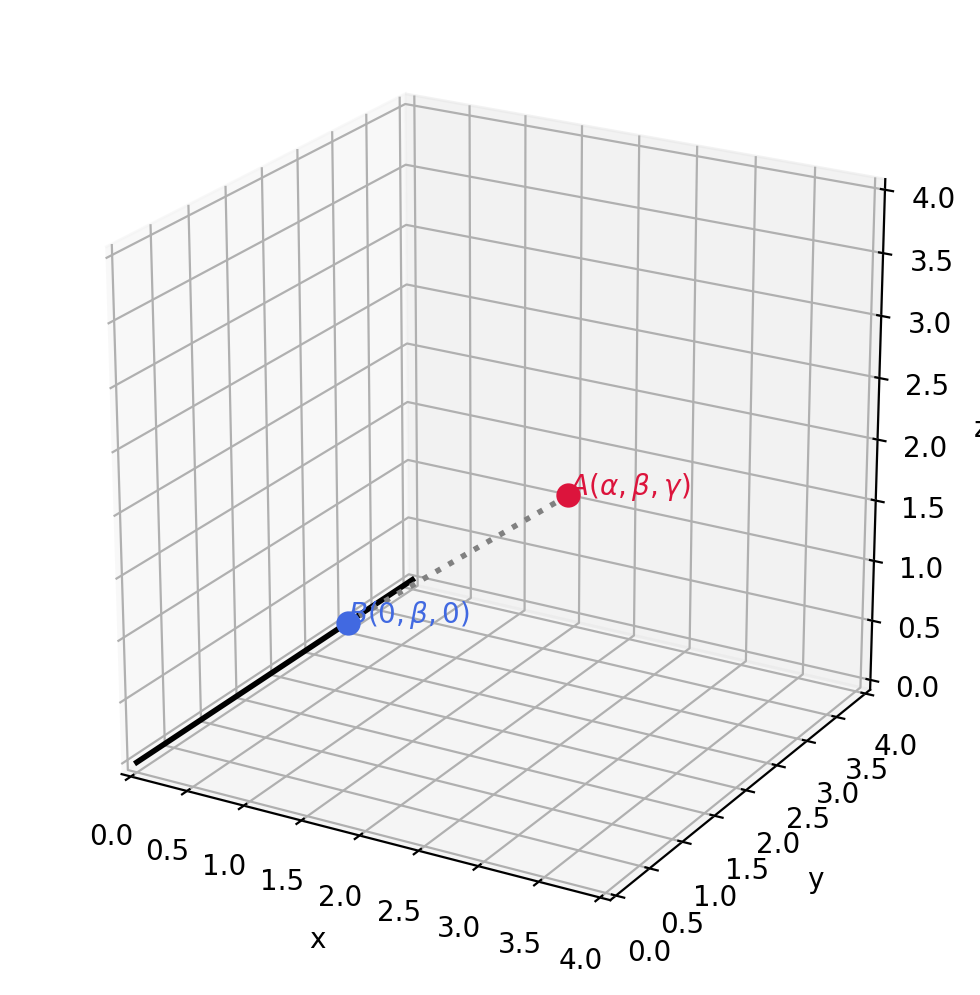
\includegraphics[width=\columnwidth]{figs/fig1.png}
    \label{fig:fig/fig1.png}
\end{figure}

\end{document}  
